\chapter{Introduction}
\section{Overview}
%https://nsdsguidelines.paris21.org/node/291
%https://papers.ssrn.com/sol3/papers.cfm?abstract_id=2622220


%markets:
%https://link.springer.com/article/10.1007/s10551-010-0402-8
%https://www.oecd-ilibrary.org/content/paper/5k49dfg9fb6d-en
%https://www.worldbank.org/en/topic/fragilityconflictviolence/overview

%problem statement/Hook
Between 1990 and 2015, the share of Africans living in absolute poverty fell from 54\% to 41\% \citep{Beegle2019}. However, given the reductions in poverty elsewhere in the world, the proportion of the world's poor who live in Africa has increased in that time period; and because of population increase in the continent, the absolute number of Africans living in poverty has also increased.  Moreover, the poverty rates within Africa haven't declined uniformly across countries, with some countries faring worse than others. The World Bank expects that by 2030, up to two thirds of the world's extremely poor live in Fragile Conflict-affected settings \citep{WorldBank2019}. However, the fact that the global poor are increasingly concentrated in a limited number of countries does not make this a localized issue: instability in one country may have effects throughout the region through increased numbers of refugees and proliferation of armed groups. Such flows may even destabilize countries further away. Climate change is expected to increase this instability further \citep{Burke2009}.

This makes understanding the dynamics of poverty in these countries of crucial importance in reducing poverty worldwide. The constituent chapters of this dissertation aim to contribute to our knowledge of these dynamics. I present micro-level evidence from Sierra Leone, Cameroon and the Democratic Republic of the Congo (DRC).


\section{Theoretical Framework}
Figure \ref{intro:fig:framework} outlines the relationships between the main topics of this dissertation. On the right-hand side, there are two indicators for development: human rights and (agricultural) productivity. On the left, there are three risks and opportunities: violent conflict, markets, and development aid. These risks and opportunities do not translate directly in development outcomes; rather, they are mediated through social capital and institutions.

\begin{figure}[htb]
  \centering
  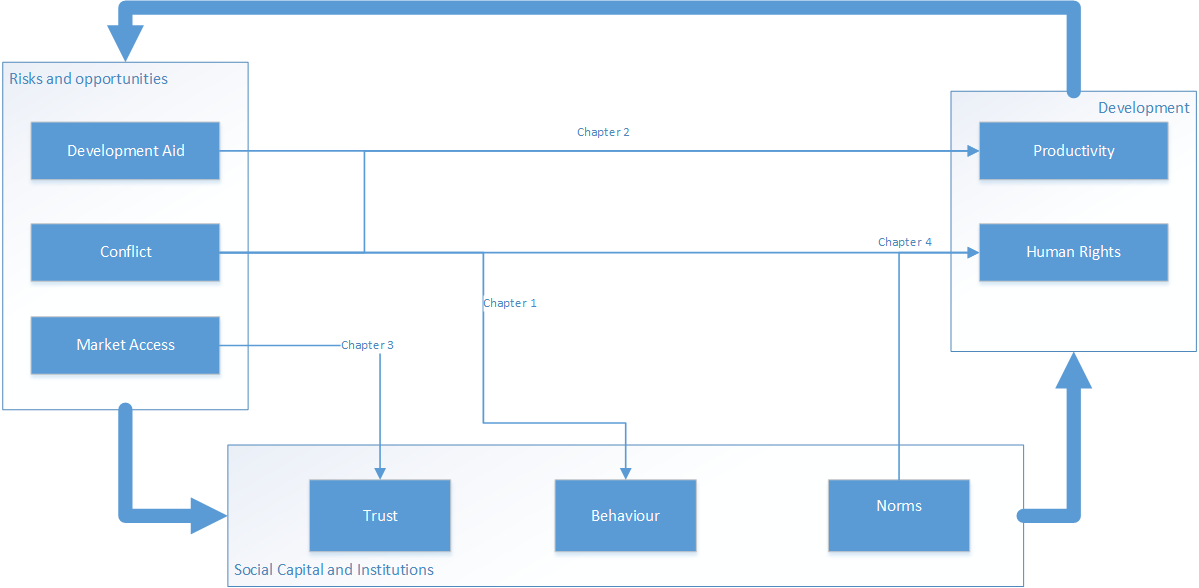
\includegraphics[width=0.8\linewidth]{"\git/thesis/analysis/introduction/figures/conceptual_framework.png"}
  \caption{Conceptual Framework}
  \label{intro:fig:framework}
\end{figure}

\subsection{Risks and Opportunities}\
As for the risks and opportunities to development I consider, the first is violent conflict. \citet{Collier2003} has labelled conflict ``Development in Reverse'', clearly indicating the risk conflicts poses to development. The 2011 World Development Report was titled Conflict, Security, and Development, further underscoring the importance of violent conflict poses in shaping development outcomes \citep{WorldBank2011}. Aside from the human rights violations that are inherent to violent conflict, other consequences include: decreased economic activity \citep{Collier1999} deforestation \cite[e.g.][]{Connectiona}, long-term incidence of domestic violence \citep[e.g.][]{LaMattina2017, Muller2019}, (mental) health problems \cite[e.g.][]{Smith2002, Iqbal2006a,Akresh2011} and food insecurity \cite[e.g.][]{Lecoutere2005, Verwimp2012}. However, some effects which may have some benefit to long-term development have been described, such as increased collective action \citep{Bellows2009b}, political participation \citep{Blattman2009a} and increased pro-social behaviour \citep{Voors2012a}.

This thesis includes insights from data from two post-conflict countries in Africa: Sierra Leone and DRC. The conflicts have had far-reaching effects. In Chapter \ref{chap:slfootball}, I examine some of the impacts that conflict has had on the behaviour of youths in Sierra Leone. Chapters \ref{chap:n2a_impact} and \ref{chap:congogbv} are set in DRC. The former focuses on agricultural productivity, which has suffered from the conflict; while the latter focuses on women's rights.

Next, I consider an opportunity for development: markets. Markets provide opportunities for exchange and specialization, which can boost economic development. At the national level, trade is seen as a promising way to increase productivity in developing economies. Dutch development aid, for example, has a large focus on the complementarities between trade and development as a way of increasing investments and thus productivity \citep[see e.g.][]{Zoomers2014}. Aside these impacts on the national level, increased access to markets have been shown to have effects at the local and individual level as well: markets are associated with trust \citep{Tu2010,Fischer2008}; increased rationality \citep{List2008,Cecchi2013,Braga2009} and decreases in risk aversion \citep{Melesse2015}. This corresponds with findings that from large-scale societies (which include markets) engage more in pro-social behaviour \cite{Henrich2005,Henrich2010}. These national and individual effects make that markets are an important consideration in analysing the development process. 

Chapter \ref{chap:cameroontrust} expands on this literature on the effects of markets on behaviour. Specifically, in the chapter I analyse how trust is shaped by the presence of local markets. The effect markets have mean they are more than a conduit for buying and selling goods, but can have deep impacts on societies.

%put in for development aid vs institutional reform: https://www.aeaweb.org/articles/pdf/doi/10.1257/jel.44.4.973
Thirdly, I consider development aid. At the turn of the century, the Millennium Development Goals were adopted in the hopes that the world's poorest countries (particularly in Africa) could be lifted out of poverty with a large-scale international effort. The underlying assumption was that a core challenge to African economies were adverse geographical conditions which hinder growth; ambitious investments by the international development community could then help increase agricultural productivity and decrease the impact of tropical diseases \citep{Sachs2005}. This push came out of disappointment with the levels of growth in the 1990s, when the World Bank and the IMF preached "stabilize, privatize and liberalize" \citep{Rodrik2006a}. However, an increase in the levels of development aid was not the only response to this disappointment: concurrently there was doubt about development aid's capability to achieve meaningful growth. \citet{Easterly2007} labels Development Assistance a ``mistake'', claiming that ``we don't know what actions achieve development''. A large literature has since sprung up that aims to fill exactly that knowledge gap and find out which development interventions work, and which don't. Improvements in statistical techniques and data collection methods have allowed development economists to get more accurate assessments of the impact of aid programs. Academics and development NGOs have embraced methods such as Randomized Controlled Trials (RCTs) to find out what works and what doesn't \citep[see e.g.][]{Bannerjee2011}.  

This dissertation follows in this tradition. Chapter \ref{chap:n2a_impact} is about the impact evaluation of an agricultural intervention, and both Chapters \ref{chap:cameroontrust} and \ref{chap:congogbv} were funded by being smaller parts of similar impact evaluations. This reflects the increased amount of field research that is being funded, allowing economists to more accurately determine what actions work for development.

\subsection{Social Capital and Institutions}
The impact that these risks and opportunities can have differs across countries. Some countries have been better able to exploit the advantages markets offer than others; one conflict-affected country rebounds more quickly than another (compare for example the fortunes of Rwanda and the DRC). The key factor that sets apart countries that are successful in avoiding risk and capitalizing on opportunities is, is their institutional environment \citep{Rodrik2004,Acemoglu2000}. This term is used to describe the rules and norms that shape (economic) life. It covers crucial things such as protection of property rights and equal treatment by the law \citep{Acemoglu2005}. Such good institutions  foster development by incentivizing innovation. However, the relationship between institutions and development does not run in one direction. While institutions cause growth \citep{Acemoglu2000}, the economic growth that accompanies development also allows for better institutions. It is possible that countries could enter a virtuous cycle, where improved institutional quality enhances growth, which improves institutional quality \citep{Voors2011}.

%
It is important to note that such institutions do not only include the formal rules and organizations which organize our lives; it includes informal arrangements shaped by the relations and networks between people as well. Insofar as these relations and networks provide value, they are termed social capital \citep[see for a more detailed discussion of the definition of the term][]{Putnam2001}. Especially in poorer countries, social capital plays an important role in facilitating economic activity \citep{Knack1997}. In such countries, social capital may be a substitute for formal institutions by providing insurance and securing property rights. 

This insight, that social behaviours substitute for formal institutions in facilitating development, suggests that is not just international and national factors that drive development. Rather, relationships and behaviours at the local level may play and important role in shaping outcomes. This means that micro-level data collection is of importance for studying development. This dissertation contributes to this, by studying the links between behaviour and conflict (Chapter \ref{chap:slfootball}) and between behaviour and markets (Chapter \ref{chap:cameroontrust}).

\subsection{Development}
As for development, I focus on agricultural productivity and human rights. I focus on agricultural production, as the poorest of the world often depend on subsistence agriculture. Furthermore, agricultural productivity is seen as a necessary precondition for further, economy-wide, productivity improvements \cite{WorldBank2008}. However, a focus on productivity is too narrow to fully capture the problems associated with poverty. Productivity gains mean little in the face of widespread human rights violations. Human dignity is a crucial part of development. In addition to agricultural productivity, I focus on human rights as well; in particular women's rights.

\section{Research Questions and outline}
Chapters \ref{chap:slfootball} through \ref{chap:congogbv} each discuss a different aspect of the framework presented above. The questions they answer are as follows.
\begin{enumerate}
	\item What is the relationship between conflict and competitive behaviour? (Chapter \ref{chap:slfootball});
	\item What is the effect of input subsidies on novel technology adoption? (Chapter \ref{chap:n2a_impact});
	\item What is the effect of market access on trusting behaviour (Chapter \ref{chap:cameroontrust}); and,
	\item What are the drivers of sexual and gender-based violence in Eastern Congo (Chapter \ref{chap:congogbv}).
\end{enumerate}

Following these, there are concluding remarks, synthesizing the lessons learned from each of these chapters.

%bibliography, this is needed for bibtex
\clearpage 
\bibliographystyle{chicago}
%path to .bib file (e.g. automatically exported by mendeley) DO NOT include the file extension!
\bibliography{\onedrive/Literatuur/Bibtex/Thesis}